\setcounter{section}{1}
\section{Eigenwertproblem}

Betrachten wir zunächst eine lineare Abbildung gegeben durch \( x \mapsto Ax \) mit \( A \in \mathbb{C}^{n \times n} \). Wie wir bereits in der Linearen Algebra I sahen, kann diese Abbildung analog zu einer Funktion interpretiert werden. Die Abbildung nimmt einen Vektor \( x \) und bildet ihn auf den Vektor \( x' = Ax \) ab. 

\begin{figure*}[h!]
    \centering
    \tikzset{every picture/.style={line width=0.75pt}} %set default line width to 0.75pt        
    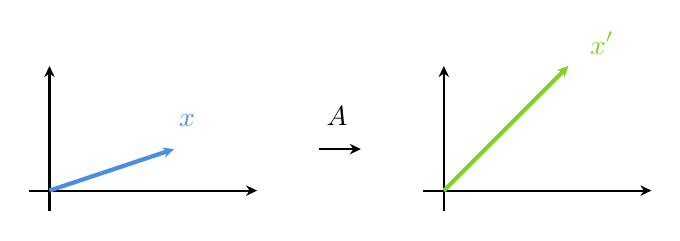
\begin{tikzpicture}[x=0.75pt,y=0.75pt,yscale=-1,xscale=1]
        %uncomment if require: \path (0,300); %set diagram left start at 0, and has height of 300
        %Straight Lines [id:da8939676934517575] 
        \draw    (180,120) -- (287,120) ;
        \draw [shift={(290,120)}, rotate = 180] [fill={rgb, 255:red, 0; green, 0; blue, 0 }  ][line width=0.08]  [draw opacity=0] (5.36,-2.57) -- (0,0) -- (5.36,2.57) -- (3.56,0) -- cycle    ;
        %Straight Lines [id:da19182460919202415] 
        \draw    (190,130) -- (190,63) ;
        \draw [shift={(190,60)}, rotate = 90] [fill={rgb, 255:red, 0; green, 0; blue, 0 }  ][line width=0.08]  [draw opacity=0] (5.36,-2.57) -- (0,0) -- (5.36,2.57) -- (3.56,0) -- cycle    ;
        %Straight Lines [id:da07596756347672651] 
        \draw    (370,120) -- (477,120) ;
        \draw [shift={(480,120)}, rotate = 180] [fill={rgb, 255:red, 0; green, 0; blue, 0 }  ][line width=0.08]  [draw opacity=0] (5.36,-2.57) -- (0,0) -- (5.36,2.57) -- (3.56,0) -- cycle    ;
        %Straight Lines [id:da052479533418790525] 
        \draw    (380,130) -- (380,63) ;
        \draw [shift={(380,60)}, rotate = 90] [fill={rgb, 255:red, 0; green, 0; blue, 0 }  ][line width=0.08]  [draw opacity=0] (5.36,-2.57) -- (0,0) -- (5.36,2.57) -- (3.56,0) -- cycle    ;
        %Straight Lines [id:da5667352567230661] 
        \draw [color={rgb, 255:red, 74; green, 144; blue, 226 }  ,draw opacity=1 ] [line width=1.5]  (190,120) -- (247.15,100.95) ;
        \draw [shift={(250,100)}, rotate = 161.57] [fill={rgb, 255:red, 74; green, 144; blue, 226 }  ,fill opacity=1 ][line width=0.08]  [draw opacity=0] (5.36,-2.57) -- (0,0) -- (5.36,2.57) -- (3.56,0) -- cycle    ;
        %Straight Lines [id:da4153575187828108] 
        \draw    (320,100) -- (337,100) ;
        \draw [shift={(340,100)}, rotate = 180] [fill={rgb, 255:red, 0; green, 0; blue, 0 }  ][line width=0.08]  [draw opacity=0] (5.36,-2.57) -- (0,0) -- (5.36,2.57) -- (3.56,0) -- cycle    ;
        %Straight Lines [id:da8411456264053829] 
        \draw [color={rgb, 255:red, 126; green, 211; blue, 33 }  ,draw opacity=1 ] [line width=1.5]  (380,120) -- (437.88,62.12) ;
        \draw [shift={(440,60)}, rotate = 135] [fill={rgb, 255:red, 126; green, 211; blue, 33 }  ,fill opacity=1 ][line width=0.08]  [draw opacity=0] (5.36,-2.57) -- (0,0) -- (5.36,2.57) -- (3.56,0) -- cycle    ;

        % Text Node
        \draw (251,82) node [anchor=north west][inner sep=0.75pt]  [color={rgb, 255:red, 74; green, 144; blue, 226 }  ,opacity=1 ] [align=left] {$\displaystyle x$};
        % Text Node
        \draw (322,78) node [anchor=north west][inner sep=0.75pt] [align=left] {$\displaystyle A$};
        % Text Node
        \draw (449,42) node [anchor=north west][inner sep=0.75pt]  [color={rgb, 255:red, 74; green, 144; blue, 226 }  ,opacity=1 ] [align=left] {$\displaystyle \textcolor[rgb]{0.49,0.83,0.13}{x'}$};
    \end{tikzpicture}
\end{figure*}

Wir fragen uns nun, ob es bestimmte Eingabevektoren \( x \) gibt, welche durch die Abbildung \( x \mapsto Ax \) nur um einen Faktor \( \lambda \) gestreckt bzw.\ gestaucht werden. 

\begin{figure*}[h!]
    \centering
    \tikzset{every picture/.style={line width=0.75pt}} %set default line width to 0.75pt        
    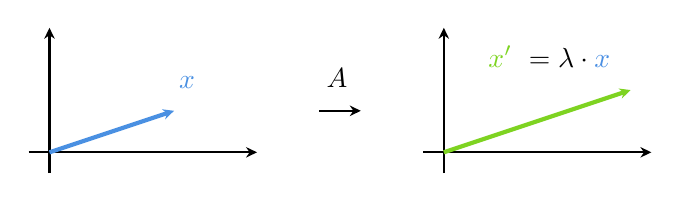
\begin{tikzpicture}[x=0.75pt,y=0.75pt,yscale=-1,xscale=1]
        %uncomment if require: \path (0,300); %set diagram left start at 0, and has height of 300

        %Straight Lines [id:da8939676934517575] 
        \draw    (180,120) -- (287,120) ;
        \draw [shift={(290,120)}, rotate = 180] [fill={rgb, 255:red, 0; green, 0; blue, 0 }  ][line width=0.08]  [draw opacity=0] (5.36,-2.57) -- (0,0) -- (5.36,2.57) -- (3.56,0) -- cycle    ;
        %Straight Lines [id:da19182460919202415] 
        \draw    (190,130) -- (190,63) ;
        \draw [shift={(190,60)}, rotate = 90] [fill={rgb, 255:red, 0; green, 0; blue, 0 }  ][line width=0.08]  [draw opacity=0] (5.36,-2.57) -- (0,0) -- (5.36,2.57) -- (3.56,0) -- cycle    ;
        %Straight Lines [id:da07596756347672651] 
        \draw    (370,120) -- (477,120) ;
        \draw [shift={(480,120)}, rotate = 180] [fill={rgb, 255:red, 0; green, 0; blue, 0 }  ][line width=0.08]  [draw opacity=0] (5.36,-2.57) -- (0,0) -- (5.36,2.57) -- (3.56,0) -- cycle    ;
        %Straight Lines [id:da052479533418790525] 
        \draw    (380,130) -- (380,63) ;
        \draw [shift={(380,60)}, rotate = 90] [fill={rgb, 255:red, 0; green, 0; blue, 0 }  ][line width=0.08]  [draw opacity=0] (5.36,-2.57) -- (0,0) -- (5.36,2.57) -- (3.56,0) -- cycle    ;
        %Straight Lines [id:da5667352567230661] 
        \draw [color={rgb, 255:red, 74; green, 144; blue, 226 }  ,draw opacity=1 ] [line width=1.5]  (190,120) -- (247.15,100.95) ;
        \draw [shift={(250,100)}, rotate = 161.57] [fill={rgb, 255:red, 74; green, 144; blue, 226 }  ,fill opacity=1 ][line width=0.08]  [draw opacity=0] (5.36,-2.57) -- (0,0) -- (5.36,2.57) -- (3.56,0) -- cycle    ;
        %Straight Lines [id:da4153575187828108] 
        \draw    (320,100) -- (337,100) ;
        \draw [shift={(340,100)}, rotate = 180] [fill={rgb, 255:red, 0; green, 0; blue, 0 }  ][line width=0.08]  [draw opacity=0] (5.36,-2.57) -- (0,0) -- (5.36,2.57) -- (3.56,0) -- cycle    ;
        %Straight Lines [id:da06992950235433282] 
        \draw [color={rgb, 255:red, 126; green, 211; blue, 33 }  ,draw opacity=1 ]  [line width=1.5] (380,120) -- (467.15,90.95) ;
        \draw [shift={(470,90)}, rotate = 161.57] [fill={rgb, 255:red, 126; green, 211; blue, 33 }  ,fill opacity=1 ][line width=0.08]  [draw opacity=0] (5.36,-2.57) -- (0,0) -- (5.36,2.57) -- (3.56,0) -- cycle    ;

        % Text Node
        \draw (251,82) node [anchor=north west][inner sep=0.75pt]  [color={rgb, 255:red, 74; green, 144; blue, 226 }  ,opacity=1 ] [align=left] {$\displaystyle x$};
        % Text Node
        \draw (322,78) node [anchor=north west][inner sep=0.75pt] [align=left] {$\displaystyle A$};
        % Text Node
        \draw (400,67) node [anchor=north west][inner sep=0.75pt] [align=left] {$\displaystyle \textcolor[rgb]{0.49,0.83,0.13}{x'\ } = \lambda \cdot \textcolor[rgb]{0.29,0.56,0.89}{x}$};
    \end{tikzpicture}
\end{figure*}

Wir wissen also, dass in diesem Fall für eine Abbildung, gegeben durch \( x \mapsto Ax \), folgendes gelten muss: \( Ax = x' = \lambda \cdot x \). Daraus können wir die allgemeine Eigenwertgleichung ableiten:

\begin{equation}
    Ax = \lambda x.
    \label{eq:eigenwertgleichung}
\end{equation}

Der Vektor \(x \) welcher durch die Abbildung nur gestreckt bzw.\ gestaucht wird, nennt sich Eigenvektor. Der Faktor \( \lambda \), um welchen der Vektor gestreckt bzw.\ gestaucht wird, nennen wir Eigenwert.

\subsection{Eigenwerte}

Wir suchen nun ein \( \lambda \), sodass \( Ax = \lambda x \) gilt. (Wir suchen nur nichttriviale Lösungen \(x \neq 0\)). Durch Umstellen von (\ref{eq:eigenwertgleichung})  erhalten wir ein homogenes lineares Gleichungssystem der Form

\begin{equation}
    (A - \lambda I) x = 0.
    \label{eq:eigenwertgleichung_homogen}
\end{equation}

Wann hat dieses HLGS nur nichttriviale Lösungen? 

\begin{tcolorbox}[colback=white, colframe=blue!50, title=Erinnerung aus der Linearen Algebra I]
    Folgende Aussagen sind für \( A^{n \times n} \) äquivalent:
    \begin{itemize}
        \item Das homogene LGS \( Ax = 0 \) besitzt nur die triviale Lösung 
        \item det\( (A) \neq 0 \)
    \end{itemize}
\end{tcolorbox}

Demnach hat das HLGS nichttriviale Lösungen genau dann wenn 

\begin{equation*}
    \text{det}(A - \lambda I) = 0
\end{equation*}

Mit dieser Gleichung können wir nun \( \lambda \) bestimmen.

\subsubsection*{Beispiel}

Sei \( A = \begin{pmatrix} 3 & 0 & 0 \\ 5 & -6 & 0 \\ 0 & 1 & 3 \end{pmatrix} \), bestimme alle Eigenwerte \( \lambda_i \) von \( A \).

\vspace{1\baselineskip}

\begin{equation*}
    \text{det}(A - \lambda I) = \text{det} \left[ \begin{pmatrix} 3 & 0 & 0 \\ 5 & -6 & 0 \\ 0 & 1 & 3 \end{pmatrix} - \lambda \begin{pmatrix} 1 & 0 & 0 \\ 0 & 1 & 0 \\ 0 & 0 & 1 \end{pmatrix}\right] = \text{det} \begin{pmatrix} 3-\lambda & 0 & 0 \\ 5 & -6-\lambda & 0 \\ 0 & 1 & 3-\lambda \end{pmatrix} = 0
\end{equation*}

\begin{equation*}
    \begin{aligned}
        (3 - \lambda)(-6 - \lambda)(3 - \lambda) = 0 \\[1em]
        \lambda_1 = 3,\ \lambda_2 = 3,\ \lambda_3 = -6
    \end{aligned}
\end{equation*}

Das Polynom \( p_A := \text{det}(A - \lambda I) \) heisst charakteristisches Polynom. Wenn \( A \in \mathbb{C}^{n \times n} \), dann ist \( p_A(\lambda) \) ein Polynom vom Grad \( n \). In unserem Beispiel ist der Eigenwert 3 eine doppelte Nullstelle des charakteristischen Polynoms. Wir sagen dann, dass die algebraische Vielfachheit des Eigenwertes 3 gleich 2 ist. Für die Matrix von oben bedeutet das

\begin{equation*}
    \begin{aligned}
        \lambda_{1,2} &= 3 &\text{hat die algebraische Vielfachheit}\ 2 \\
        \lambda_3 &= -6 &\text{hat die algebraische Vielfachheit}\ 1
    \end{aligned}
\end{equation*}

\vspace{1\baselineskip}

Merkmale und Definitionen von Eigenvektoren einer Matrix \( A \in \mathbb{C}^{n \times n} \):

\begin{itemize}
    \item \( A \) hat mindestens einen Eigenwert \( \lambda \in \mathbb{C} \)
    \item \( A \) hat höchstens \( n \) Eigenwerte \( \lambda \in \mathbb{C} \)
    \item \( A \) hat genau \( n \) Eingenwerte \( \lambda \in \mathbb{C} \), wenn man die Vielfachheit zählt
    \item die Menge aller Eigenwerte von \( A \) heisst Spektrum von \( A \) 
    \item Zwei Matrizen \( A, B \in \mathbb{C}^{n \times n} \) heissen ähnlich, wenn für eine reguläre Matrix \( T \in \mathbb{C}^{n \times n} \) gilt: \( B = T^{-1} A T \). Ferner haben \( A \) und \( B \) dann:
    \begin{itemize}
        \item dasselbe charakteristische Polynom
        \item dieselben Eigenwerte mit denselben algebraischen Vielfachheiten
        \item dasselbe Spektrum
        \item dieselbe Determinante
    \end{itemize}
\end{itemize}

\subsection{Eigenvektoren}

Wir wissen nun wie wir die Eigenwerte \( \lambda \) erhalten, nun müssen wir noch die dazugehörigen Eigenvektoren berechnen. Das heisst den Vektor \( x \) bestimmen, für welchen gilt:

\begin{equation*}
    Ax = \lambda x \quad (x \neq 0)
\end{equation*}

Das Problem kann wieder zu einem homogenen LGS der Form (\ref{eq:eigenwertgleichung_homogen}) umgeschrieben werden. Nun setzten wir einen der Eigenwerte ein und lösen das HLGS.\ Demnach sind die Eigenvektoren immer mit einem Eigenwert verknüpft.

\subsubsection*{Beispiel}
Sei \( A = \begin{pmatrix} 3 & 0 & 0 \\ 5 & -6 & 0 \\ 0 & 1 & 3 \end{pmatrix} \) mit den Eigenwerten \( \lambda_{1,2} = 3, \lambda_3 = -6 \). Bestimme die Eigenvektoren \( v_{\lambda_1}, v_{\lambda_2}, v_{\lambda_3} \) von \( A \).

\vspace{1\baselineskip}

Für den ersten Eigenvektor müssen wir folgendes HLGS lösen:

\begin{equation*}
    v_{\lambda_1}: (A - \lambda_1 I) x = (A - 3I) x = 0. 
\end{equation*}

Mit der gegebenen Matrix ergibt sich

\begin{equation*}
        \begin{pmatrix} 0 & 0 & 0 \\ 5 & -9 & 0 \\ 0 & 1 & 0 \end{pmatrix} x = 0. 
\end{equation*}

Welches die Lösung

\begin{equation*}
        x_3 = t \in \mathbb{R};\ x_2 = 0;\ x_1 = 0 
\end{equation*}

besitzt und somit in den folgenden Eigenvektor resultiert:

\begin{equation*}
        v_{\lambda_1} = \begin{pmatrix} 0 \\ 0 \\ 1 \end{pmatrix}.
\end{equation*}

Da die Eigenwerte \( \lambda_1 = \lambda_2 \) sind, ist der Eigenvektor \( v_{\lambda_2} \) identisch zu \( v_{\lambda_1} \). Für den dritten Eigenvektor müssen wir folgendes HLGS lösen:

\begin{equation*}
    v_{\lambda_3}: (A - \lambda_3 I) x = (A + 6I) x = 0.
\end{equation*}

Mit der gegebenen Matrix ergibt sich

\begin{equation*}
        \begin{pmatrix} 9 & 0 & 0 \\ 5 & 0 & 0 \\ 0 & 1 & 9 \end{pmatrix} x = 0.
\end{equation*}

Welches die Lösung

\begin{equation*}
        x_1 = 0;\ x_2 = -9 x_3 
\end{equation*}

besitzt und somit in den folgenden Eigenvektor resultiert:

\begin{equation*}
        v_{\lambda_3} = \begin{pmatrix} 0 \\ -9 \\ 1 \end{pmatrix}.
\end{equation*}

Da wir bei der Berechnung für Eigenvektoren ein HLGS mit det \(= 0 \) lösen, wird es immer unendlich viele Lösungen für \( (A-\lambda I) x = 0 \) geben. D.h.\ jede mögliche Linearkombination von Eigenvektoren von einem Eigenwert ist auch wieder ein Eigenvektor zum gleichen Eigenwert. Der dadurch aufgespannte Vektorraum ist dann ein Unterraum von \( \mathbb{C}^n \) und nennt sich Eigenraum. Eigenräume werden mit \( E_{\lambda_i} \) bezeichnet.

\subsubsection*{Beispiel}

Sei \( A = \begin{pmatrix} 2 & 1 & 1 \\ 1 & 2 & 1 \\ 1 & 1 & 2 \end{pmatrix} \) mit den Eigenwerten \( \lambda_{1,2} = 1, \lambda_3 = 4 \). Bestimme die Eigenvektoren von \( A \).

\vspace{1\baselineskip}

Genau wie oben müssen wir ein HLGS lösen.

\begin{equation*}
    E_{\lambda_1} = E_{\lambda_2} = E_{1}: (A - \lambda_1 I) x = (A - 1I) x = 0.
\end{equation*}

\begin{equation*}
    \begin{pmatrix} 1 & 1 & 1 \\ 1 & 1 & 1 \\ 1 & 1 & 1 \end{pmatrix} x = 0 \ \xrightarrow[]{\text{Gauss}} \begin{pmatrix} 1 & 1 & 1 \\ 0 & 0 & 0 \\ 0 & 0 & 0 \end{pmatrix} x = 0.
\end{equation*}

\vspace{0.25\baselineskip}

Nun haben wir zwei freie Parameter:

\begin{equation*}
    x_3 = t;\ x_2 = s;\ x_1 = -s - t \quad s, t \in \mathbb{R}.
\end{equation*}

Der resultierende Eigenraum zum Eigenwert 1 ist somit

\begin{equation*}
    E_1 = \text{span} \left\{ \begin{pmatrix} -1 \\ 1 \\ 0 \end{pmatrix}, \begin{pmatrix} -1 \\ 0 \\ 1 \end{pmatrix} \right\}.
\end{equation*}

\( E_4 \) kann auf die gleiche Weise berechnet werden.

\vspace{\baselineskip}

In diesem Beispiel ist also der Eigenraum \( E_1 \) zum Eigenwert 1 ein zweidimensionaler Unterraum. Die Dimension des Eigenraums dim\( (E_{\lambda_i}) \) heisst geometrische Vielfachheit des Eigenwertes \( \lambda_i \). In unserem Beispiel ist also die geometrische Vielfachheit von \( \lambda_1 =  2 \). Die geometrische Vielfachheit ist immer gleich der Anzahl freier Parameter des HLGS \( (A - \lambda I)x = 0 \). Allgemein ist immer zu beachten, dass für einen Eigenwert \( \lambda \) der Matrix \( A \in \mathbb{C}^{n \times n} \) gelten muss:

\begin{equation*}
    1 \leq \text{geom. Vielfachheit}(\lambda) \leq \text{alg. Vielfachheit}(\lambda) \leq n.
\end{equation*}